\begin{figure}[ht]
\centering
\resizebox{\textwidth}{!}{%
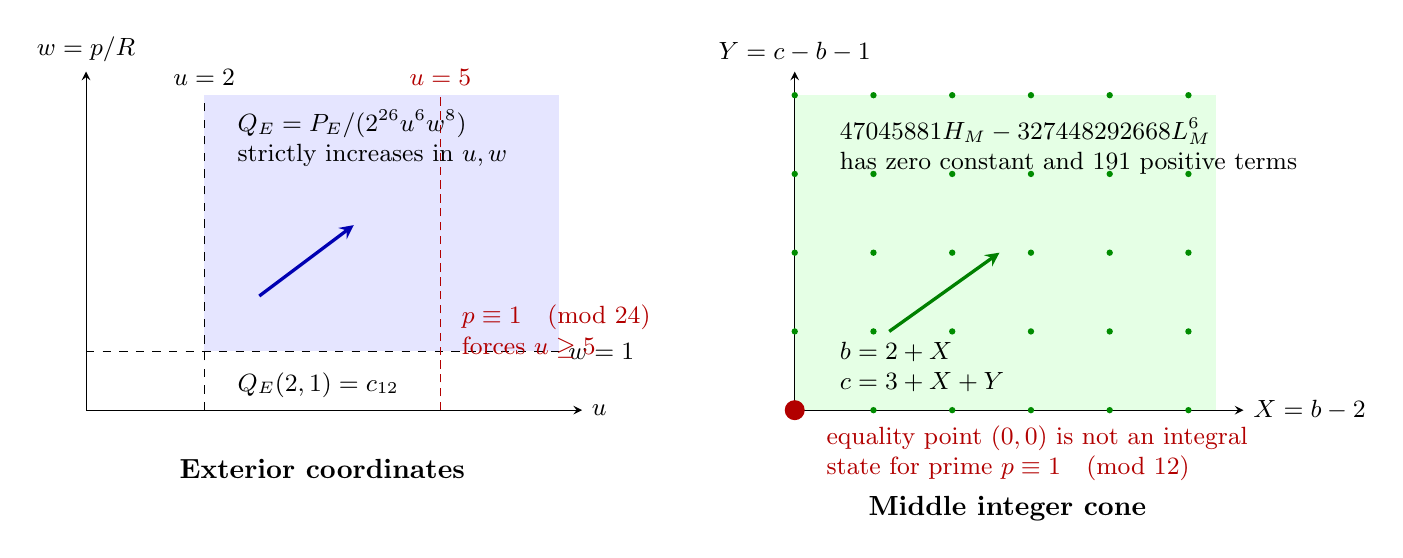
\begin{tikzpicture}[font=\small,>=stealth]
  % Exterior cone.
  \begin{scope}[xshift=0cm]
    \draw[->] (0,0) -- (6.3,0) node[right] {$u$};
    \draw[->] (0,0) -- (0,4.3) node[above] {$w=p/R$};
    \fill[blue!10] (1.5,0.75) rectangle (6,4);
    \draw[dashed] (0,0.75) -- (6,0.75) node[right] {$w=1$};
    \draw[dashed] (1.5,0) -- (1.5,4) node[above] {$u=2$};
    \draw[densely dashed,red!70!black] (4.5,0) -- (4.5,4) node[above] {$u=5$};
    \draw[->,very thick,blue!70!black] (2.2,1.45) -- (3.4,2.35);
    \node[align=left,anchor=west] at (1.8,3.45)
      {$Q_E=P_E/(2^{26}u^6w^8)$\\strictly increases in $u,w$};
    \node[align=left,anchor=west] at (1.8,0.32)
      {$Q_E(2,1)=c_{12}$};
    \node[align=left,anchor=west,red!70!black] at (4.65,1.0)
      {$p\equiv1\pmod{24}$\\forces $u\ge5$};
    \node[font=\bfseries] at (3,-0.75) {Exterior coordinates};
  \end{scope}

  % Middle cone.
  \begin{scope}[xshift=9cm]
    \draw[->] (0,0) -- (5.7,0) node[right] {$X=b-2$};
    \draw[->] (0,0) -- (0,4.3) node[above] {$Y=c-b-1$};
    \fill[green!10] (0,0) rectangle (5.35,4);
    \foreach \x in {0,...,5}{\foreach \y in {0,...,4}{\fill[green!55!black] (\x,\y) circle (1.15pt);}}
    \draw[->,very thick,green!50!black] (1.2,1.0) -- (2.6,2.0);
    \draw[fill=white,very thick,red!70!black] (0,0) circle (3pt);
    \node[align=left,anchor=west] at (0.45,3.35)
      {$47045881H_M-327448292668L_M^6$\\has zero constant and $191$ positive terms};
    \node[align=left,anchor=west] at (0.45,0.55)
      {$b=2+X$\\$c=3+X+Y$};
    \node[align=left,anchor=west,red!70!black] at (0.28,-0.55)
      {equality point $(0,0)$ is not an integral\\state for prime $p\equiv1\pmod{12}$};
    \node[font=\bfseries] at (2.7,-1.25) {Middle integer cone};
  \end{scope}
\end{tikzpicture}
}%
\caption{The two exact coordinate domains used in the global sign proof.  The
blue and green regions are certificate domains; actual Erd\H{o}s--Straus
witnesses are the arithmetic points satisfying the displayed gates and
integrality conditions.  The exterior lower bound is approached at the dashed
boundary $w=1$, which is excluded by $R<p$.  The middle comparison is strict at
every admissible lattice point because its only equality point would require
$a=6p/19$.}
\label{fig:coordinate-domains}
\end{figure}
